\begin{tikzpicture}
\begin{axis} [
     title={},
     width=\textwidth,
     height=.25\textheight,
     xlabel={\footnotesize \textbf{Failures}},
     ylabel={\footnotesize \textbf{Frequency}},
     bar width = 4pt,
     ybar = .01cm,
     xmin=0.0, xmax=5,
     ymin=0.0, ymax=140,
     x tick label style={font=\tiny},
     y tick label style={font=\tiny},
     xtick={1,2,3,4},
     xticklabels={VQA - Fail, Grounding - Fail, Both - Fail, Both - Success},
     y label style={at={(axis description cs:0.05,.5)},anchor=south},
     ymajorgrids=false,
     xmajorgrids=false,
     legend style={
			at={(0.5,-0.3)},
			anchor=north,
			legend columns=5,
            }
] 

\addplot[color=blue, fill=blue, area legend] coordinates{(1, 45) (2, 12) (3, 87) (4, 6)};
\addplot[color=blue!60, fill=blue!60,  area legend] coordinates {(1, 5) (2, 11) (3, 132) (4, 2)};
\addplot[color=blue!30, fill=blue!30,  area legend] coordinates {(1, 62) (2, 6) (3, 76) (4, 6)};
\addplot[color=blue!40, fill=blue!10,  area legend] coordinates {(1, 69) (2, 0) (3, 80) (4, 1)};
\addplot[color=blue!40, fill=blue!2,  area legend] coordinates {(1, 8) (2, 18) (3, 124) (4, 0)};

\addplot[color=red!20, fill=red!20,  area legend] coordinates {(1, 17) (2, 48) (3, 74) (4, 11)};
\addplot[color=red!60, fill=red!60,  area legend] coordinates {(1, 20) (2, 35) (3, 89) (4, 6)};
\addplot[color=red, fill=red,  area legend] coordinates {(1, 24) (2, 61) (3, 49) (4, 16)};

\legend{\textbf{OMG-Llava (7B)}, \textbf{Llava-G (7B)}, \textbf{LISA (7B)}, \textbf{GLaMM (7B)}, \textbf{GLaMM$\dagger$ (7B)}, \textbf{Llava (13B)}, \textbf{Llava (7B)}, \textbf{Cambrian (8B)}}

\end{axis}
\end{tikzpicture}